% Created by tikzDevice version 0.10.1 on 2018-02-09 14:35:34
% !TEX encoding = UTF-8 Unicode
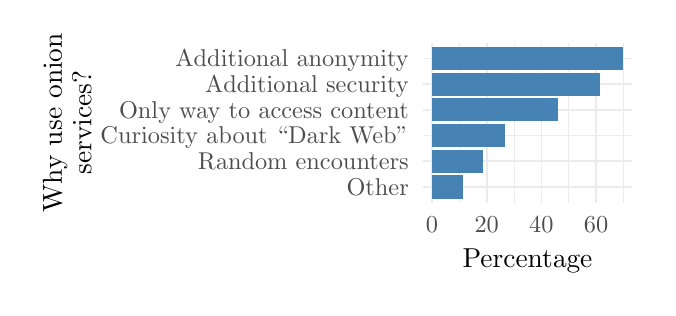
\begin{tikzpicture}[x=1pt,y=1pt]
\definecolor{fillColor}{RGB}{255,255,255}
\path[use as bounding box,fill=fillColor,fill opacity=0.00] (0,0) rectangle (224.04, 93.95);
\begin{scope}
\path[clip] (142.68, 30.77) rectangle (218.54, 88.45);
\definecolor{drawColor}{gray}{0.92}

\path[draw=drawColor,line width= 0.3pt,line join=round] (156.00, 30.77) --
	(156.00, 88.45);

\path[draw=drawColor,line width= 0.3pt,line join=round] (175.75, 30.77) --
	(175.75, 88.45);

\path[draw=drawColor,line width= 0.3pt,line join=round] (195.50, 30.77) --
	(195.50, 88.45);

\path[draw=drawColor,line width= 0.3pt,line join=round] (215.26, 30.77) --
	(215.26, 88.45);

\path[draw=drawColor,line width= 0.6pt,line join=round] (142.68, 36.35) --
	(218.54, 36.35);

\path[draw=drawColor,line width= 0.6pt,line join=round] (142.68, 45.66) --
	(218.54, 45.66);

\path[draw=drawColor,line width= 0.6pt,line join=round] (142.68, 54.96) --
	(218.54, 54.96);

\path[draw=drawColor,line width= 0.6pt,line join=round] (142.68, 64.26) --
	(218.54, 64.26);

\path[draw=drawColor,line width= 0.6pt,line join=round] (142.68, 73.57) --
	(218.54, 73.57);

\path[draw=drawColor,line width= 0.6pt,line join=round] (142.68, 82.87) --
	(218.54, 82.87);

\path[draw=drawColor,line width= 0.6pt,line join=round] (146.12, 30.77) --
	(146.12, 88.45);

\path[draw=drawColor,line width= 0.6pt,line join=round] (165.88, 30.77) --
	(165.88, 88.45);

\path[draw=drawColor,line width= 0.6pt,line join=round] (185.63, 30.77) --
	(185.63, 88.45);

\path[draw=drawColor,line width= 0.6pt,line join=round] (205.38, 30.77) --
	(205.38, 88.45);
\definecolor{fillColor}{RGB}{70,130,180}

\path[fill=fillColor] (146.12, 32.17) rectangle (157.37, 40.54);

\path[fill=fillColor] (146.12, 41.47) rectangle (164.49, 49.84);

\path[fill=fillColor] (146.12, 50.77) rectangle (172.55, 59.15);

\path[fill=fillColor] (146.12, 60.08) rectangle (191.48, 68.45);

\path[fill=fillColor] (146.12, 69.38) rectangle (206.84, 77.75);

\path[fill=fillColor] (146.12, 78.68) rectangle (215.09, 87.06);
\end{scope}
\begin{scope}
\path[clip] (  0.00,  0.00) rectangle (224.04, 93.95);
\definecolor{drawColor}{gray}{0.30}

\node[text=drawColor,anchor=base east,inner sep=0pt, outer sep=0pt, scale=  0.88] at (137.73, 33.32) {Other};

\node[text=drawColor,anchor=base east,inner sep=0pt, outer sep=0pt, scale=  0.88] at (137.73, 42.63) {Random encounters};

\node[text=drawColor,anchor=base east,inner sep=0pt, outer sep=0pt, scale=  0.88] at (137.73, 51.93) {Curiosity about ``Dark Web''};

\node[text=drawColor,anchor=base east,inner sep=0pt, outer sep=0pt, scale=  0.88] at (137.73, 61.23) {Only way to access content};

\node[text=drawColor,anchor=base east,inner sep=0pt, outer sep=0pt, scale=  0.88] at (137.73, 70.54) {Additional security};

\node[text=drawColor,anchor=base east,inner sep=0pt, outer sep=0pt, scale=  0.88] at (137.73, 79.84) {Additional anonymity};
\end{scope}
\begin{scope}
\path[clip] (  0.00,  0.00) rectangle (224.04, 93.95);
\definecolor{drawColor}{gray}{0.30}

\node[text=drawColor,anchor=base,inner sep=0pt, outer sep=0pt, scale=  0.88] at (146.12, 19.76) {0};

\node[text=drawColor,anchor=base,inner sep=0pt, outer sep=0pt, scale=  0.88] at (165.88, 19.76) {20};

\node[text=drawColor,anchor=base,inner sep=0pt, outer sep=0pt, scale=  0.88] at (185.63, 19.76) {40};

\node[text=drawColor,anchor=base,inner sep=0pt, outer sep=0pt, scale=  0.88] at (205.38, 19.76) {60};
\end{scope}
\begin{scope}
\path[clip] (  0.00,  0.00) rectangle (224.04, 93.95);
\definecolor{drawColor}{RGB}{0,0,0}

\node[text=drawColor,anchor=base,inner sep=0pt, outer sep=0pt, scale=  0.99] at (180.61,  7.44) {Percentage};
\end{scope}
\begin{scope}
\path[clip] (  0.00,  0.00) rectangle (224.04, 93.95);
\definecolor{drawColor}{RGB}{0,0,0}

\node[text=drawColor,rotate= 90.00,anchor=base,inner sep=0pt, outer sep=0pt, scale=  0.99] at ( 12.32, 59.61) {Why use onion};

\node[text=drawColor,rotate= 90.00,anchor=base,inner sep=0pt, outer sep=0pt, scale=  0.99] at ( 23.01, 59.61) {services?};
\end{scope}
\end{tikzpicture}
